\section[The bounty from the SVD]{The bounty from \svdl}
The elegance of the SVD blossoms when we examine the domain and the codomain in terms of contributions from the target matrix to the $\X{}$ and $\Y{}$ matrices shown in table \eqref{tab:vecs}.

\subsection{The row space: home of the solution}
The domain is $\real{2}$ and is resolved into two orthonormal vectors. The first vector comes from the first row vector (the first column in the matrix transpose) and becomes  $\X{}_{*,1}$. The orthogonal complement is \textit{constructed} based upon the first vector. The result becomes $\X{}_{*,2}$.

\subsection{The column space: home of the measurements}
The codomain is $\real{3}$ and requires three orthonormal vectors. The first vector comes from the first column vector in the target matrix and becomes  $\Y{}_{*,1}$. The orthogonal complement is \textit{constructed} based upon the first vector. The result becomes $\Y{}_{*,2}$ and $\Y{}_{*,3}$.

These orthogonal complements are also called null spaces\index{null spaces!orthogonal complements}. When the matrix acts upon a vector from the null space it produces a zero vector. For example
\begin{equation}
  \begin{split}
     \Aexample  \mat{c}{1\\1}      = \mat{c}{0\\0\\0} = \zero,\\
     \Atexample \mat{c}{0\\1\\1}   = \mat{c}{0\\0}    = \zero,\\
     \Atexample \mat{r}{2\\1\\-1}  = \mat{c}{0\\0}    = \zero.
  \end{split}
\end{equation}
The null spaces are named to identity the target matrix. This produces a result that unsettles some when the first learn the theory. When the vectors the matrix $\A{}$ operates on vectors from Because the zero vector in the domain is created by the matrix $\A{T}$.
\begin{table}[htdp]
\begin{center}
\begin{tabular}{cccc}
         & operates on  &\\
  matrix & vectors from & to produce & vectors form\\\hline
  $\A{}$  & $\rng{\A{T}}^{\perp}$ & $\mat{c}{0\\0\\0}$ & $\nll{\A{}}$\\
  $\A{T}$ & $\rng{\A{}}^{\perp}$  & $\mat{c}{0\\0}$    & $\nll{\A{T}}$
\end{tabular}
\end{center}
\label{tab:02:null}
\caption[Null spaces and orthogonal complements to range spaces]{Null spaces and orthogonal complements to range spaces.}
\end{table}%

\begin{equation}
  \begin{split}
     \rng{\A{T}}^{\perp} &\equiv \nll{\A{}},\\
     \rng{\A{}}^{\perp}  &\equiv \nll{\A{T}},\\
  \end{split}
\end{equation}

These relationships are shown in table \eqref{tab:vecs}.

\begin{table}[h]
\begin{center}
\begin{tabular}{cccc}
Domain & source & host & null \\ vector & vector & space & space \\\hline\hline
$\X{}_{*,1}$ & $\A{T}_{*,1}$ & $\rng{\A{T}}$ \\[3pt]
$\X{}_{*,2}$ & $\paren{\A{T}_{*,1}}^{\perp}$ & $\rng{\A{T}}^{\perp}$ & $\nll{\A{}}$\\
&\\\hline
&\\
$\Y{}_{*,1}$ & $\A{}_{*,1}$ & $\rng{\A{}}$ \\[3pt]
$\Y{}_{*,2}$ & $\paren{\A{}_{*,1}}^{\perp}$ & $\rng{\A{}}^{\perp}$ & $\nll{\A{T}}$ \\[3pt]
$\Y{}_{*,3}$ & $\paren{\A{}_{*,1}}^{\perp}$ & $\rng{\A{}}^{\perp}$ & $\nll{\A{T}}$ \\[5pt]
\end{tabular}
\end{center}
\caption[Resolving the domain and codomain into complete orthonormal systems]{Resolving the domain and codomain into complete orthonormal systems. In this pedagogical example we can see connections between the domain matrices $\X{}$ and $\Y{}$ and the inputs $\A{}$ and $\A{T}$. The \svdl \ has resolved the row and column spaces into complete domains $\real{2}$ and $\real{3}$ by resolving the orthogonal complements.}
\label{tab:vecs}
\end{table}

%%
\section{Before and after}
Consider the issue of the vector spaces before and after the SVD. The row and column spaces are the spans of the linearly independent row and column vectors. When we plot all of the row and column vectors it is clear that each vector space has one linearly independent vector.

Perhaps the shortest summary is in{tab:munificence} which shows the vector spaces for the target matrix before and after the \svdl. We were able to use the first row and column vector for the range vectors. Then the complementary null space vectors were constructed.
\begin{table}[htdp]
\begin{center}
\begin{tabular}{lll}
 & DOMAIN & CODOMAIN \\
 & (Induced by row space) & (Induced by column space) \\\hline\hline
 pre SVD: & $\spn \lst{\mat{r}{1\\-1}}$ & $\spn \lst{\mat{r}{1\\-1\\1}}$ \phantom{$\mat{c}{1\\1\\1\\1}$}\\[5pt]\hline
 post SVD:  & $\underbrace{\spn \lst{\mat{r}{1\\-1}}}_{\rng{\A{T}}} \oplus \underbrace{\spn \lst{\mat{r}{1\\1}}}_{\rng{\A{T}}^{\perp}}$ & $\underbrace{\spn \lst{\mat{r}{1\\-1\\1}}}_{\rng{\A{}}^{\phantom{T}}} \oplus \underbrace{\spn \lst{\veca,\vecb}}_{\rng{\A{}}^{\perp}}$ \\[35pt]\hline
\end{tabular}
\end{center}
\label{tab:munificence}
\caption[The SVD resolves the fundamental subspaces]{The munificence of the SVD. The target matrix has row and column spaces that are incomplete. The SVD resolves these spaces into complete, orthonormal spaces for the domain and codomain.}
\end{table}

``The completeness of a space'' may seem like an abstract term. It has a concrete meaning. For example, if the host space is $\real{2}$, then a complete space is a vector space which allows access to every point in the plane. If the vector space $\mathcal{V}$ is given as
\begin{equation}
\mathcal{V} = \spn \lst{\mat{r}{1\\-1}}
\end{equation}
then only points along the line including the origin and the point 
\begin{equation}
p=\mat{r}{1\\-1}
\end{equation}
can be accessed. For example, the points 
$$
\mat{r}{2\\-2},\ \mat{r}{3\\-3},\ \mat{r}{\pi\\-\pi},\ \sqrt{2}\mat{r}{-1\\1}
$$
are on this line. The point 
\begin{equation*}
  \mat{r}{1\\0}
\end{equation*}
is not on the line.

A problem with the target matrix is that both the row space and the column space are incomplete. Figures \eqref{fig:2d} and \eqref{fig:3d} show the incomplete row and column spaces represented by the row and column vectors of the target matrix.
\begin{figure}[htbp] %  figure placement: here, top, bottom, or page
   \centering
   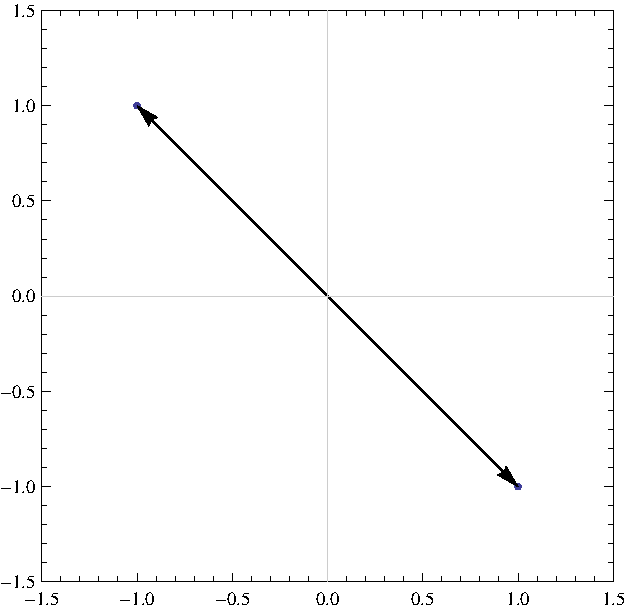
\includegraphics[ width = 2in ]{pdf/post_mortem/2d_before} \qquad
   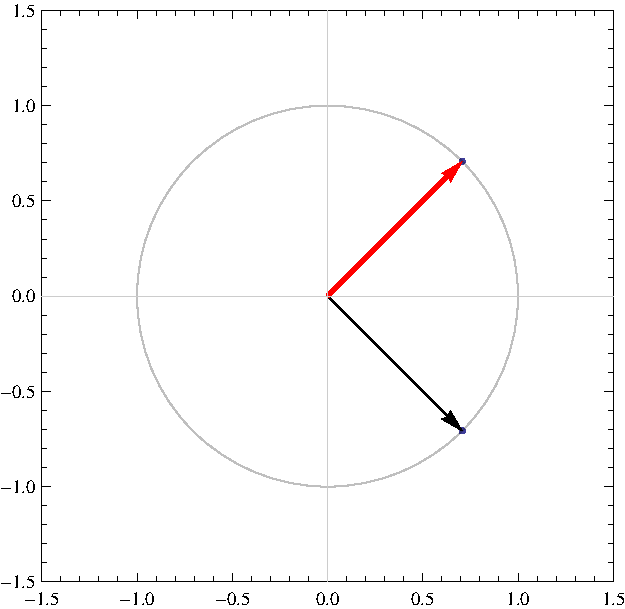
\includegraphics[ width = 2in ]{pdf/post_mortem/2d_after} 
   \caption[The row space before and after the SVD]{The row space before and after the SVD. The row vectors of the target matrix are on the left and the orthonormal resolution of the domain on the right. The null vector which completes the space is shown in red.}
   \label{fig:2d}
\end{figure}

\begin{figure}[htbp] %  figure placement: here, top, bottom, or page
   \centering
   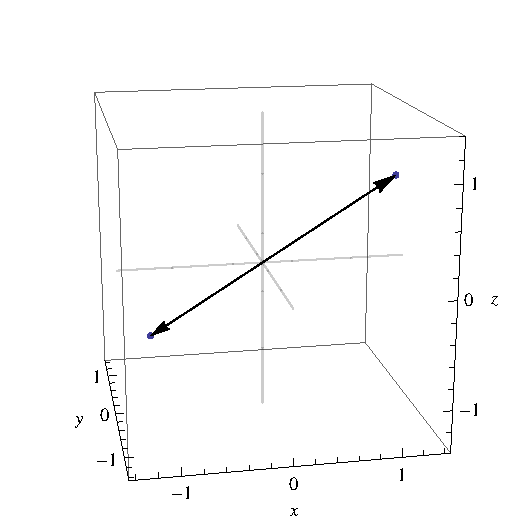
\includegraphics[ width = 2.2in ]{pdf/post_mortem/3d_before} \qquad
   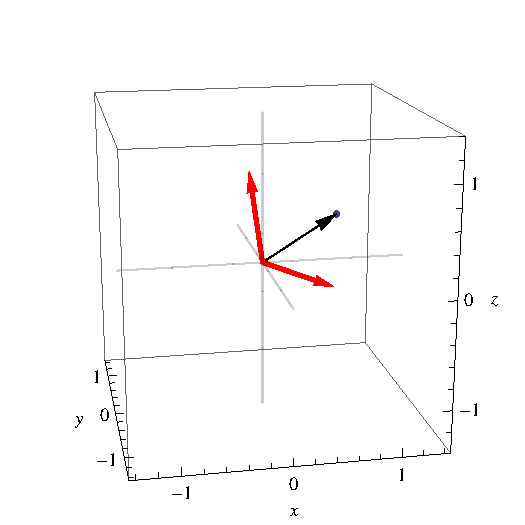
\includegraphics[ width = 2.2in ]{pdf/post_mortem/3d_after} 
   \caption[The column space before and after the SVD]{The column space before and after the SVD. Here too the column space is redundant and incomplete as seen by plotting the column vectors on the left. The orthonormal basis for the complete space is shown on the right.}
   \label{fig:3d}
\end{figure}

%%
\section{The action of the pseudoinverse}
Let's briefly touch on the issue raised in \S\eqref{sec:pi} and look at the product of a matrix and its pseudoinverse. The matrix products are these:

\begin{equation}
  \begin{array}{rcrrcl}
    \leftinv  &=& \Aexample & \Aplus &=& \rthree
    \mat{rrr}
    { 1 & 0 &  1\\
     -1 & \phantom{-}1 & -1\\
      1 & 0 &  1},\\
    \rightinv &=& \Aplus & \Aexample &=& \rtwo
    \mat{rr}
    { 1 & -1\\
     -1 & 1}.\\
  \end{array}
\end{equation}

We will look at another example in \S\eqref{lrfirst} and analyze the situation in the section on chiral inverses \S\eqref{sec:chiral} which will lead to the interpretation in terms of fundamental projectors \S\eqref{sec:orthproj}.

%%
\section{Thin SVD}
Look at the action of the $\sig{}$ matrix holding the singular values. Because of the sabot, the singular values are protected from the null spaces and interact with only the ranges. In effect these paddings prevent the null spaces from contributing the value of the target matrix. It's clear that the null vectors play no role in reconstituting the matrix $\A{}$.

%%
\subsection{An example}
In this context, it makes sense to fashion a \index{thin SVD}\textit{thin SVD} which excludes the null space vectors and the sabot. The thin $\sig{}$ matrix reduces to an $\by{\rho}{\rho}$ diagonal matrix. Using a tilde to denote the thin versions of the product matrices, the thin SVD for the matrix $\A{}$ becomes
\begin{equation}
  \begin{split}
    \A{} &= \svdthin{T},\\
    \Aexample & = \sthree \mat{r}{1\\-1\\1}\mat{c}{\sqrt{6}}\stwo\mat{cc}{1&-1}.
  \end{split}
  \label{eq:thin}
\end{equation}
The dimensions reductions for this problem are these:
$$
\begin{array}{lll}
\text{full SVD} & \svdax{T} & \by{3}{2} = \paren{\by{3}{3}}\paren{\by{3}{2}}\paren{\by{2}{2}} \\
\text{thin SVD} & \A{} = \svdthin{T} & \by{3}{2} = \paren{\by{3}{1}}\paren{\by{1}{1}}\paren{\by{1}{2}} \\
\end{array}
$$

Figure \eqref{fig:thin} displays the SVD before and after losing the null space vectors. Correlate this diagram to equation \eqref{eq:thin}.
\begin{figure}[htbp] %  figure placement: here, top, bottom, or page
   \centering
   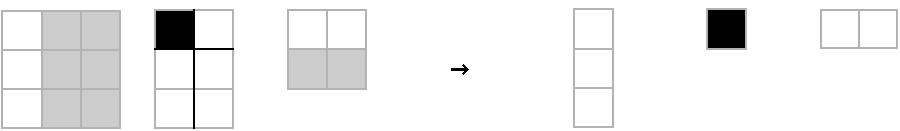
\includegraphics[ width = 5in ]{pdf/post_mortem/thin} 
   \caption[The secret to a thin SVD]{The secret to a thin SVD - lose the null spaces and the sabot. Matrices with incomplete row or column spaces are the only matrices that will shrink under the thin SVD.}
   \label{fig:thin}
\end{figure}

%%
\subsection{The general case}
As you might surmise, the dimensions and rank of the target matrix fully specify the dimensions for both the SVD and the thin SVD. The difference is the null space vectors; the lower the rank the thinner the ``thin SVD''. For a matrix 
\begin{equation}
  \A{}\in \mathbb{C}^{\by{m}{n}}_{\rho}
\end{equation}
the dimensions are given below in table \eqref{tab:bounty:thinsvd}.

\begin{table}[htdp]
\begin{center}
\begin{tabular}{llll}
SVD\quad & formulation & dimensions & size is rank\dots \\\hline
full & $\svd{*}$ & $\by{m}{n} = \paren{\by{m}{m}}\,\paren{\by{m}{n}}\,\paren{\by{n}{n}}$ & independent \\
thin & $\svdthin{*}$ & $\by{m}{n} = \paren{\by{m}{\rho}}\,\paren{\by{\rho}{\rho}}\,\paren{\by{\rho}{n}}$ & dependent 
\end{tabular}
\end{center}
\label{tab:bounty:thinsvd}
\caption[Dimensions for full and thin SVDs]{A comparison between the sizes of the component matrices for a full and thin SVD. Essentially, the thin SVD omits the null space vectors.}
\end{table}%

\endinput